\section{Overview}
\begin{figure}
    \centering
    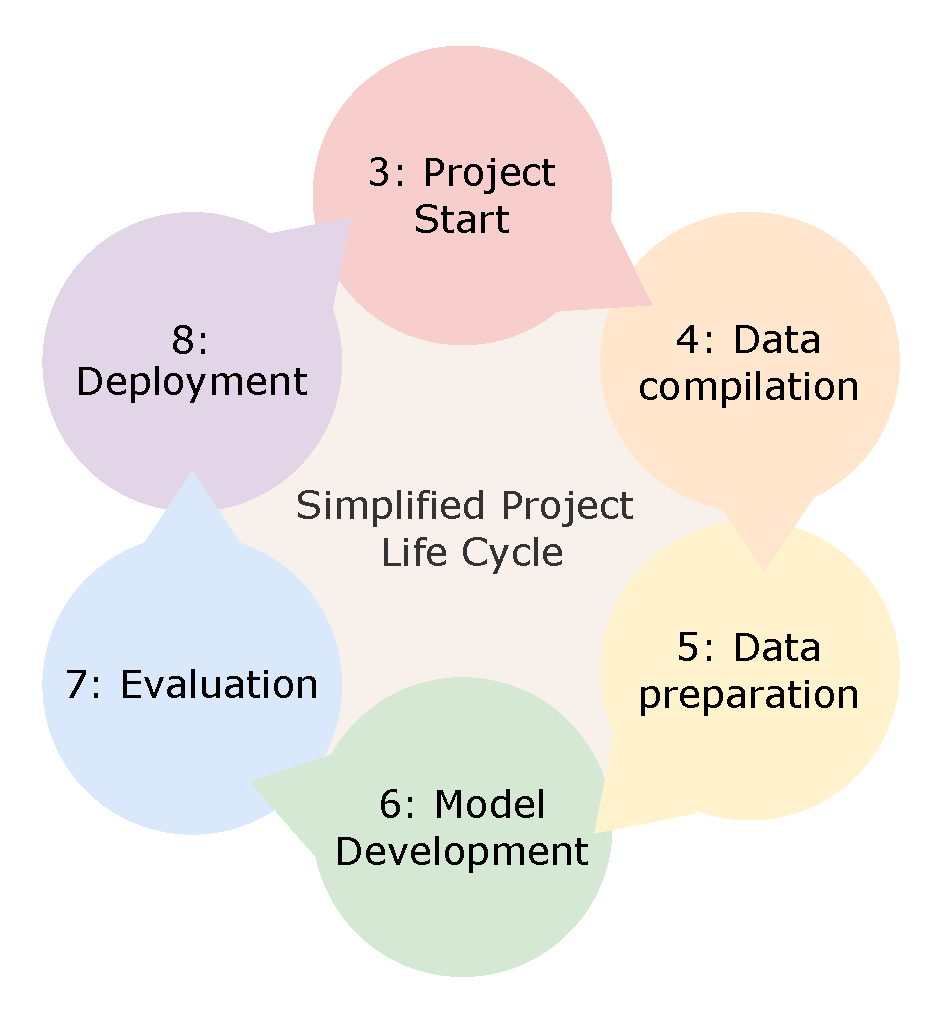
\includegraphics[scale=0.4]{whitepaperstructure.pdf}
    \caption{Diagram showing simplified project lifecycle that forms the structure of this paper.}
    \label{fig:paperstructure}
\end{figure}
%\textcolor{ForestGreen}{Eddie}
This document is structured around a (simplified) project lifecycle, depicted in \Cref{fig:paperstructure}. Our aim for this whitepaper is for it to be used as a reference guide throughout a project, rather than for post-hoc reflection. We begin in \Cref{sec:start} by outlining the importance of ethics and discussing themes relevant to the entire development life cycle.
In \Cref{sec:comp} we consider best practice for data collection and sharing.
Next, in \Cref{sec:prep} we discuss ethical aspects of data preparation, such as cleaning and labelling.
We then turn towards model development in \Cref{sec:modeldev}, focusing on questions of model design, addressing social biases and model alignment.
Following a common develop-then-test structure, we then consider ethical issues related to performance and harm evaluation in \Cref{sec:eval}.
Finally in \Cref{sec:deploy}, we examine the questions of ethics that arise in deployment contexts. You should of course adapt the order you consult these sections to your needs e.g. those finetuning an existing LLM may wish to consult \Cref{sec:modeldev} on Model Development (which has advice for model selection) before Section \hyperref[sec:comp]{4} on Data Compilation (for guidance on compiling finetuning data). However, we recommend every practitioner starts with \Cref{sec:start}, as this has vital guidance for all projects. 

At the end of each Section we give key resources, namely concrete \textcolor{ForestGreen}{do's} and \textcolor{red}{don'ts} for ethical research, relevant to that stage on the project, and tools to guide ethical work. 

%\Lexi{Overview at the moment is very short - perhaps it could fit into Section 1? Also the blue arrow of Finetuning is not very clear to me - I don't feel like it adds much. Also - is there a place that we discuss what the risks are and specifically how to mitigate them? I know others might have done this better but it is not clear where these are. } Lexi: OK happy to move forward on this
%\Eddie{Agree overview can be added to intro but keeping as separate section to section numbers remain same as in email. I have clarified in overview where mitigation lies. Risks discussed in next section. Figure updated}
%\Nik{I prefer the way they are now, it's a place where people can refer back to if they need to find their way around, but am also happy to change merge with intro}
